\chapter{Results}

\section{Baselines} \label{baselines}
\noindent In order to benchmark the various \acrshort{DRL} algorithms and test the implemented simulator, several baseline algorithms were developed:

\begin{itemize}
    \item Full Local: all \acrshort{UE}s execute their tasks locally, in terms of the decision vector $\mathcal{A}=[0_1, 0_2, ..., 0_N]$. This represents the case where the system has no offloading capabilities.
    \item Random Offload: where the offloading decision is completely random, each task is either executed locally or offloaded to one of the available \acrshort{MEC} servers randomly;
    \item Full nearest \acrshort{MEC}: all \acrshort{UE} tasks are offloaded to the nearest \acrshort{MEC} server according to Equation (\ref{distance_nm}). This represents the case of offloading to the nearest node without regarding their computation constraints and other offloading decisions. This baseline also requires knowledge of the network topology which the agent does not have.
\end{itemize}

The plan is to create several system configurations of increasing complexity. The baseline algorithms will be used in order to benchmark the quality of trained agents. It is expected that the proposed network manager will surpass their performance in all situations by making intelligent decisions taking into account computation, battery, delay and communication constraints, which are ignored by the baselines.

\section{Simple test} \label{simple_test}

To put these baselines, the agent and the simulator to the test, a simple test case was devised. In this test, there are five \acrshort{UE}s and five \acrshort{MEC} servers. The UEs and MEC servers were randomly distributed in a 2D plane with $x \in [0, 200]$ and $y \in [0, 200]$, resulting in the distribution seen in Figure \ref{example_layout}.

\begin{figure}[H]
  \centering
  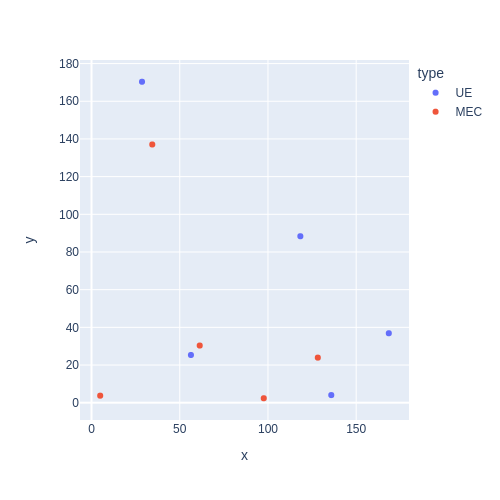
\includegraphics[width=200px]{images/example_layout.png}
  \caption{Example layout for the simple test.}  \label{example_layout}
\end{figure}

For simplicity, all \acrshort{UE}s and \acrshort{MEC} servers are considered to have the same specifications. The system's hyper-parameters were set according to the values present in Table \ref{hyperparams}. In order to test this configuration, the task parameters, $B_n$, $B_d$ and $D_n$ were sampled from uniform distributions between ($300$, $500$) Kbits, ($10$, $15$) Kbits and ($900$, $1100$) Megacyles respectivly. 

% Please add the following required packages to your document preamble:
% \usepackage[normalem]{ulem}
% \useunder{\uline}{\ul}{}
\begin{table}[H]
\centering
\begin{tabular}{|l|l|l|l|}
\hline
Variable             & Value & Variable                & Value \\ \hline
$B$&$10\times10^{6}$&$f_n^l$&$1\times10^{9}$\\
$n$&$10$&$I_n^t$&$0.5$\\
$\beta$&$-4$&$I_n^e$&$0.5$\\
$h_ul$&$100$& $P_m$&$200$\\
$h_dl$&$100$& $P_n$& $500\times10^{-3}$\\
$g_ul$&$1$&$P_n^i$&$100\times10^{-3}$\\
$g_dl$&$1$&$P_n^d$&$200\times10^{-3}$\\
$N_0$&$5\times10^{-5}$&$F_m$&$5\times10^{9}$\\
$W_{mean}$&$1$&$W_{max}$&$0$\\ \hline
\end{tabular}
\caption{System hyper-parameters.}\label{hyperparams}
\end{table}

The agent described in Section \ref{solution} was trained with the following hyper-parameters:

\begin{table}[H]
\centering
\begin{tabular}{|l|l|}
\hline
Variable & Value \\ \hline
episode length&$10$\\
learning rate, $\alpha$&$0.0001$\\
discount factor, $\gamma$&$0.99$\\
batch size&$200$\\ \hline
\end{tabular}
\caption{Training hyper-parameters.}\label{training_hyperparams}
\end{table}

Each algorithm ran for 100 episodes and an average per episode of offloading decisions is shown in Table \ref{resultstest1}.

\begin{table}[H]
\centering
\begin{tabular}{|l|l|l|}
\hline
Algorithm        & Average Reward ($R$) & Reduction\\ \hline
Full Local       & -49.47 & 96.65\%\\
Random Offload   & -9.68 & 82.89\%\\
Full nearest MEC & -2.18 & 24.06\%\\ 
Agent (A2C) & -1.66 & -\\ \hline
\end{tabular}
\caption{Average Reward ($R$) over 100 iterations.} \label{resultstest1}
\end{table}

As expected, the Full Local baseline performed the worst given that it does not make use of the \acrshort{MEC} servers computing capabilities, leading to an increased cost due to increased energy consumption and delay of the tasks. The Random Offload baseline is the second worst, given that although it gains from offloding to \acrshort{MEC} servers, it does so without any consideration for the system's configuration. From the baselines, Full nearest MEC performed the best since it takes into consideration the distance between the \acrshort{UE} and the \acrshort{MEC} server but it comes with the disadvantage of not only requiring knowledge of the network topology (positions of \acrshort{UE}s and \acrshort{MEC}s) but also not taking into account anything else. 

As expected, the proposed agent outperformed the baselines in all situations, which demonstrates that the agent is able to learn not only the topology of the network by trying out different offloading decisions but also make intelligent decisions based on computation, battery, delay and communication constraints ignored by the baselines.

\begin{figure}[H]
  \centering
  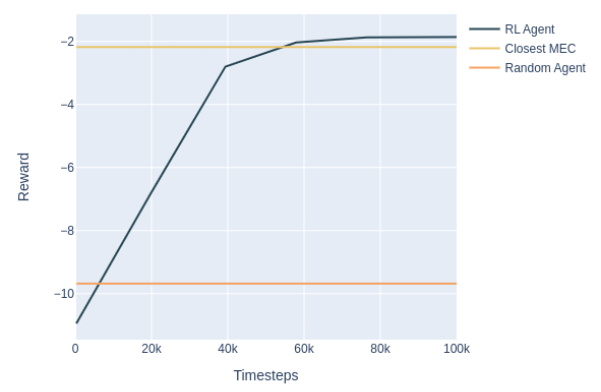
\includegraphics[width=250px]{images/5_5_training.png}
  \caption{Agent reward while training.}  \label{5_5_training}
\end{figure}

As shown in Figure \ref{5_5_training}, the agent starts with an equivelent reward to the Random Offload, which is expected since the agent has not yet learned the environment. As the agent interacts with the environment making offloading decisions (actions), it recieves state transitions and rewards. This allows it to quickly learn the system and the reward increases rapidly in the first iterations. After about 55K steps in the environment, the agent surpasses the best offloading baseline, Full nearest MEC. As expected, the reward starts to stabilize as the agent learns the final details of the system increasing slightly the final performance.

\section{Scalability and Data Efficiency} \label{scalability_data}

In this section the scalability and data efficiency of our agent is explored. Scalability in this context can be defined as the ability of the agent to learn and outperform the baselines in higher complexity problems. 

Data efficiency in this context can be defined as the ability of the agent to learn in as few possible steps as possible. While it is expected that the agent takes longer to learn in more complex problems, the complexity of the underlying policy should not grow linearly with the state and action spaces. The reason for this is that it is expected that the agent is able to generalize concepts instead of brute forcing a solution for each problem set.

Since our state space is defined as the requested tasks at each step and each task is defined by a set of 5 parameters, the complexity of the state space grows linearly with the amount of \acrshort{UE}s, \emph{N}. The size of the state space should be $N \times 5$. 

On the other side, the action space is defined as the offloading decision of each task. Given that each task can be computed locally or offloaded to one of the \acrshort{MEC} servers, \emph{M}, this gives us the option of $M + 1$ actions per task. This results in the action space growing exponentially with the amount of \acrshort{UE}s, \emph{N}, since there are $(M + 1)^N$ possible actions at each decision step.

With this in mind, the stability and data efficieny of the system can be tested by setting the system's hyper-parameters and amount of \acrshort{MEC} servers to be the same as in the simple test case and create two new test scenarios by increasing the number of \acrshort{UE}s to 10 and 20, respectively.

The UEs and MEC servers were randomly distributed in a 2D plane with $x \in [0, 200]$ and $y \in [0, 200]$, resulting in the distribution seen in Figure \ref{5_10_layout} and Figure \ref{5_20_layout}.

\begin{minipage}{0.5\textwidth}
\begin{figure}[H]
  \centering
  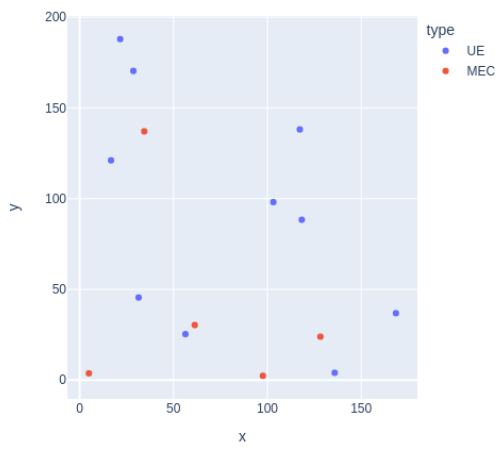
\includegraphics[width=200px]{images/5_10_layout.png}
  \caption{Test with 10 \acrshort{UE}s.}  \label{5_10_layout}
\end{figure}
\end{minipage}
\begin{minipage}{0.5\textwidth}
\begin{figure}[H]
  \centering
  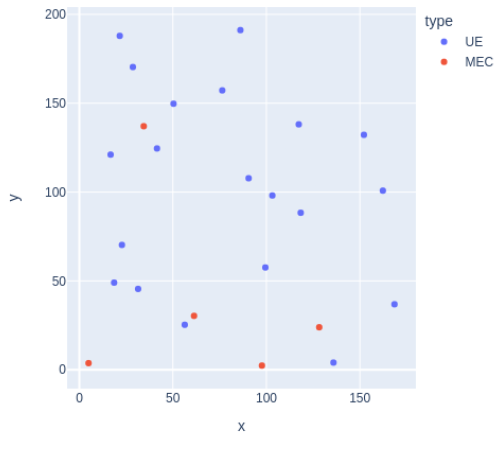
\includegraphics[width=200px]{images/5_20_layout.png}
  \caption{Test with 20 \acrshort{UE}s.}  \label{5_20_layout}
\end{figure}
\end{minipage}

\hfill \break
Each algorithm ran for 100 episodes and an average per episode of offloading decisions is shown in Table \ref{results_5_10} and Table \ref{results_5_20}.

\begin{table}[H]
\centering
\begin{tabular}{|l|l|l|}
\hline
Algorithm        & Average Reward ($R$) & Reduction\\ \hline
Full Local       & -49.50 & 94.40\%\\
Random Offload   & -10.32 & 73.14\%\\
Full nearest MEC & -3.56 & 22.17\%\\ 
Agent (A2C) & -2.77 & -\\ \hline
\end{tabular}
\caption{Average Reward ($R$) over 100 episodes with 10 \acrshort{UE}s} \label{results_5_10}
\end{table}

\begin{table}[H]
\centering
\begin{tabular}{|l|l|l|}
\hline
Algorithm        & Average Reward ($R$) & Reduction\\ \hline
Full Local       & -49.49 & 90.42\%\\
Random Offload   & -11.67 & 59.36\%\\
Full nearest MEC & -7.23 & 34.38\%\\ 
Agent (A2C) & -4.74 & -\\ \hline
\end{tabular}
\caption{Average Reward ($R$) over 100 episodes with 20 \acrshort{UE}s} \label{results_5_20}
\end{table}

As expected, the reward of the Full Local baseline stays almost the same between test environments. This happens because these tests set $W_{mean}$ to 1 and $W_{max}$ to 0, so the cost is only composed by $C_{mean}$, defined in Equation \ref{C_mean}. Since $C_{mean}$ is the average cost of each \acrshort{UE}'s task, this should not scale with the amount of \acrshort{UE}s.

The same cannot be said of the other baselines and the agent. Since the number of \acrshort{MEC}s stays the same and the number of tasks increases, the overall cost of the system increases with the amount of \acrshort{UE}s. This represents the computation constraint of the \acrshort{MEC} servers. 

These results demonstrate that the agent scales with the complexity of the system.

In order to study the data efficiency of the agent, the agent's performance while training must be analysed.


\begin{minipage}{0.5\textwidth}
\begin{figure}[H]
  \centering
  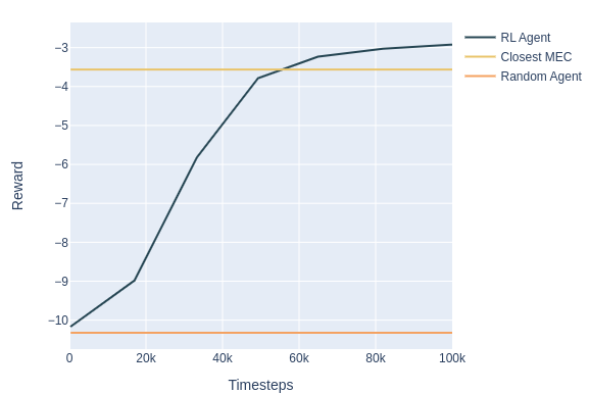
\includegraphics[width=230px]{images/5_10_training.png}
  \caption{Training with 10 \acrshort{UE}s.}  \label{5_10_training}
\end{figure}
\end{minipage}
\begin{minipage}{0.5\textwidth}
\begin{figure}[H]
  \centering
  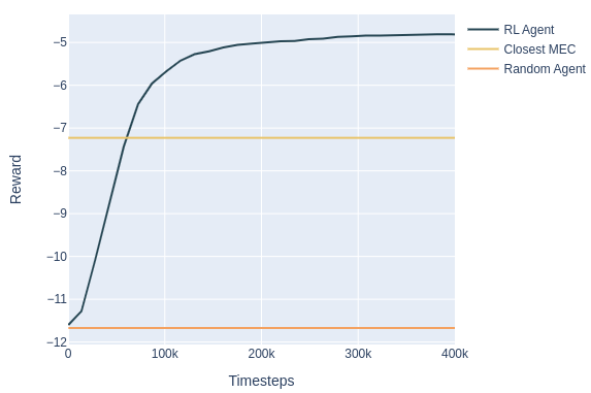
\includegraphics[width=230px]{images/5_20_training.png}
  \caption{Training with 20 \acrshort{UE}s.}  \label{5_20_training}
\end{figure}
\end{minipage}

\hfill \break
The same trend as the simple test can be observed with the two new tests in Figure \ref{5_10_training} and Figure \ref{5_20_training}. The agents starts with an equivelent reward to the Random Offload, then it quickly learns the system and the reward increases rapidly in the first iterations. After about 55K steps in both environments, the agent surpasses the best offloading baseline, Full nearest MEC. As expected, the reward starts to stabilize as the agent learns the final details of the system increasing slightly the final performance.

This confirms that the agent is data efficient, meaning that even when the system's state space increases linearly and the action space increases exponentially, the agent is able to generalize concepts achieving a good performance. It does this with almost the same number of interactions with the system proving it is finding a strategy without brute forcing a solution.

\section{Robustness and Stability} \label{robustness_stability}

In this section the robustness and stability of our agent is explored. Robustness in this context can be defined as the ability of the agent to learn and outperform the baselines in environments with different network conditions and heterogeneous computation capabilities. 

Stability in this context can be defined has the ability of the agent to not diverge or collapse while training. This means that its performance should improve as it interacts with the environment and after learning a strategy it should not forget it, collapsing the system's performance.

In order to test the system's robustness to changing network conditions, a new test case is devised by setting the system hyper-parameters to the values present in Table \ref{new_hyperparams}.

\begin{table}[H]
\centering
\begin{tabular}{|l|l|l|l|}
\hline
Variable             & Value & Variable                & Value \\ \hline
$B$&$10\times10^{6}$&$f_n^l$&$0.75\times10^{9}$\\
$n$&$10$&$I_n^t$&$0.25$\\
$\beta$&$-4$&$I_n^e$&$0.75$\\
$h_ul$&$50$& $P_m$&$100$\\
$h_dl$&$50$& $P_n$& $250\times10^{-3}$\\
$g_ul$&$0.5$&$P_n^i$&$50\times10^{-3}$\\
$g_dl$&$0.5$&$P_n^d$&$100\times10^{-3}$\\
$N_0$&$3\times10^{-5}$&$F_m$&$2.5\times10^{9}$\\
$W_{mean}$&$1$&$W_{max}$&$0$\\ \hline
\end{tabular}
\caption{New system hyper-parameters.}\label{new_hyperparams}
\end{table}

By setting the number of \acrshort{UE}s to 10 and the number of \acrshort{MEC}s to 5, they were randomly distributed in a 2D plane with $x \in [0, 200]$ and $y \in [0, 200]$, resulting in the distribution seen in Figure \ref{robust_test}.

\begin{figure}[H]
  \centering
  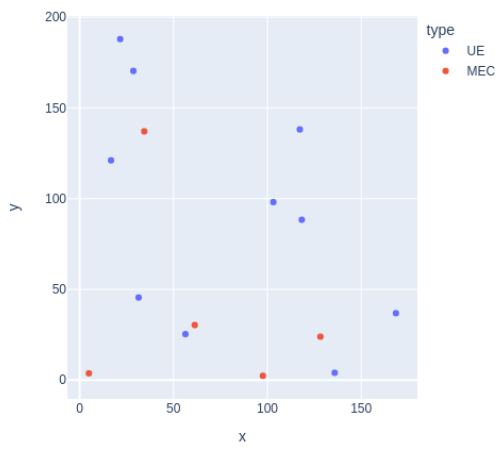
\includegraphics[width=200px]{images/5_10_layout.png}
  \caption{Robustness test layout.}  \label{robust_test}
\end{figure}

Each algorithm ran for 100 episodes and an average per episode of offloading decisions is shown in Table \ref{robust_table}.

\begin{table}[H]
\centering
\begin{tabular}{|l|l|l|}
\hline
Algorithm        & Average Reward ($R$) & Reduction\\ \hline
Full Local       & -31.31 & 84.92\%\\
Random Offload   & -9.14 & 48.35\%\\
Full nearest MEC & -6.81 & 30.62\%\\ 
Agent (A2C) & -4.72 & -\\ \hline
\end{tabular}
\caption{Average Reward ($R$) over 100 episodes of robustness test.} \label{robust_table}
\end{table}

As expected the reward values of all the algorithms differ from previous tests since the system hyper-parameters that are used to calculate the reward function are different.

The same cost reduction trends can be observed in this new environment, showing that the agent is able to learn the system's behaviour independently of the network conditions.

\begin{figure}[H]
  \centering
  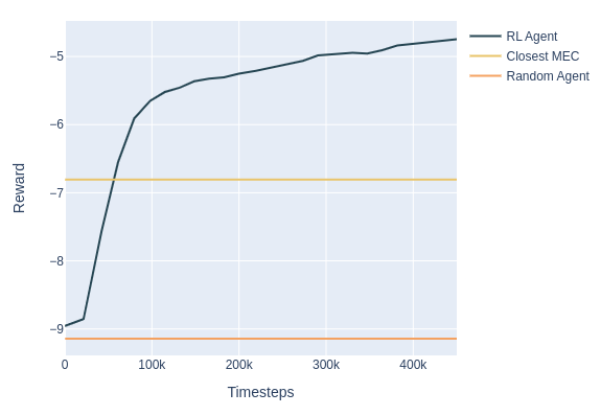
\includegraphics[width=250px]{images/5_10_training_new.png}
  \caption{Training in robustness test.}  \label{robust_training}
\end{figure}

As shown in Figure \ref{robust_training}, the agent's performance while training follows a similar trend to previous tests. The agent starts with an equivelent reward to the Random Offload, then it quickly learns the system and the reward increases rapidly in the first iterations. After about 55K steps, the agent surpasses the best offloading baseline, Full nearest MEC. As expected, the reward starts to stabilize as the agent learns the final details of the system, slightly increasing the final performance.

The other component of robustness that must be tested is robustness to heterogeneous computation capabilities of \acrshort{UE}s and \acrshort{MEC} servers. To test this, a new test case is devised by resetting the system hyper-parameters to the values present in Table \ref{hyperparams} but instead of setting $f^l_n$ and $F_m$ to a fixed value, they are set to a value randomly sampled from a set of values, $f = \{0.25, 0.5, 0.75, 1\} \times 10^9$ and $F = \{2.5, 5, 7, 10\} \times 10^9$, respectively.

By setting the number of \acrshort{UE}s to 10 and the number of \acrshort{MEC}s to 5, they were randomly distributed in a 2D plane with $x \in [0, 200]$ and $y \in [0, 200]$, resulting in the distribution seen in Figure \ref{hetero_test}.

\begin{figure}[H]
  \centering
  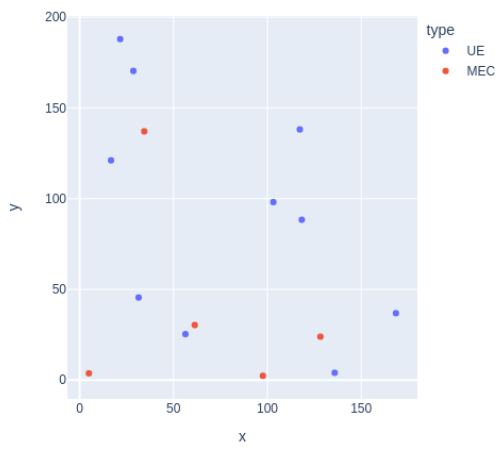
\includegraphics[width=200px]{images/5_10_layout.png}
  \caption{Heterogeneous test layout.}  \label{hetero_test}
\end{figure}

Each algorithm ran for 100 episodes and an average per episode of offloading decisions is shown in Table \ref{hetero_table}.

\begin{table}[H]
\centering
\begin{tabular}{|l|l|l|}
\hline
Algorithm        & Average Reward ($R$) & Reduction\\ \hline
Full Local       & -33.56 & 89.55\%\\
Random Offload   & -8.80 & 60.16\%\\
Full nearest MEC & -5.04 & 30.39\%\\ 
Agent (A2C) & -3.51 & -\\ \hline
\end{tabular}
\caption{Average Reward ($R$) over 100 episodes of heterogeneous test.} \label{hetero_table}
\end{table}

As presumed, the reward values of all the algorithms differ from previous tests since the system computation capabilities that are used to calculate the reward function are different.

Although the ordering of the algorithm performances stays the same in this test case, the cost reduction of our agent in comparison to the Full nearest MEC is higher. With a reported 30.39\% improvement, while the equivelant homogeneous test had an improvement of 22.17\%. This makes sense given that the Full nearest MEC only takes into account the distance of \acrshort{UE}s to \acrshort{MEC}s and not their computation capabilities. This in turn leads to worse load balancing when the computation capabilities of the \acrshort{UE}s and \acrshort{MEC}s are not all the same.

The agent on the other hand is able to learn the system's network topology and make offloading decisions that better load balance the required tasks. 

By analysing all training curves, it is clear that the agent is stable and its reward does not diverge or collapse while trainnig, even when ran for millions of iterations.

\begin{figure}[H]
  \centering
  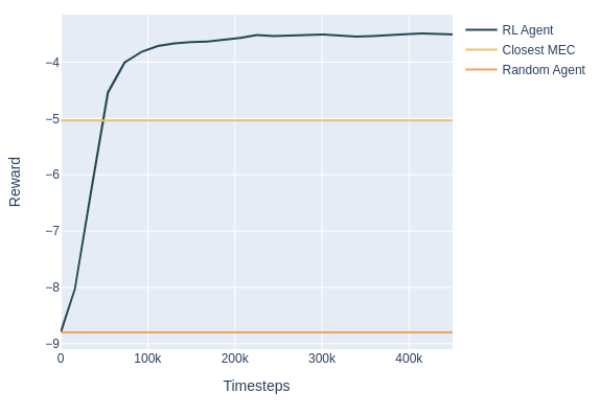
\includegraphics[width=250px]{images/5_10_training_hetero.png}
  \caption{Training in heterogeneous environment.}  \label{hetero_training}
\end{figure}

As shown in Figure \ref{hetero_training}, the agent's performance while training follows a similar trend to previous tests. The agent starts with an equivelent reward to the Random Offload, then it quickly learns the system and the reward increases rapidly in the first iterations. After about 50K steps, the agent surpasses the best offloading baseline, Full nearest MEC. As expected, the reward starts to stabilize as the agent learns the final details of the system increasing slightly the final performance.

\section{Reward function weights} \label{reward_section}

This section focuses on studying the effect of the cost function importance weights on the agent's overall and worst-case performance.

To test this, five new test cases were created by setting the system hyper-parameters to the values present in Table \ref{hyperparams} but instead of setting $W_{mean}$ to 1 and $W_{max}$ to 0, they are set to $(1, 0.75, 0.5, 0.25, 0)$ and $(0, 0.25, 0.5, 0.75, 1)$, respectively.

By setting the number of \acrshort{UE}s to 10 and the number of \acrshort{MEC}s to 5, they were randomly distributed in a 2D plane with $x \in [0, 200]$ and $y \in [0, 200]$, resulting in the distribution seen in Figure \ref{weight_test}.

\begin{figure}[H]
  \centering
  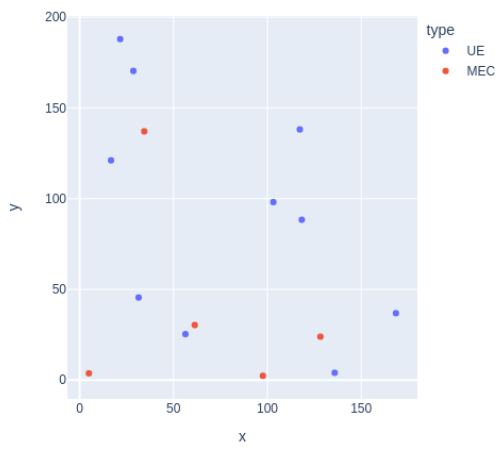
\includegraphics[width=200px]{images/5_10_layout.png}
  \caption{Weight test layout.}  \label{weight_test}
\end{figure}

Each combination of the cost function ran for 100 episodes and an average per episode of offloading decisions is shown in Table \ref{weight_table}.

\begin{table}[H]
\centering
\begin{tabular}{|l|l|l|l|}
\hline
$\{W_{mean}, W_{max}\}$ & Overall Cost & Worst Cost & Difference \\ \hline
$\{1, 0\}$       & 2.72 & 4.04 & 1.32\\
$\{0.75, 0.25\}$  & 2.97 & 3.84  & 0.87\\
$\{0.5, 0.5\}$ & 3.22 & 3.53 & 0.31\\ 
$\{0.25, 0.75\}$ & 3.52 & 3.81 & 0.29\\ 
$\{0, 1\}$ & 3.81 & 3.78 & -0.03 \\ \hline
\end{tabular}
\caption{Agent performance over 100 episodes of weight tests.} \label{weight_table}
\end{table}

As the weights shift from prioritizing overall performance to prioritizing worst-case performance, the agent's overall cost increases while the worst-case cost decreases. While the agent outperforms the best baseline with every weight distribution, it learns to make offloading decisions that prioritize the worst-case performance at the expense of overall system performance. With this in mind, the process of picking the best weight distribution would involve trying to determine the maximum cost allowed per \acrshort{UE} and shifthing the weight distribution in favour of $W_{max}$, trying to maximize $W_{mean}$ while still meeting the maximum allowed cost.
